\documentclass{homework}
\author{Tomás Pérez}
\class{Mathematical Biostatistics Boot Camp 1}
\date{\today}
\title{Theory \& Notes}

\graphicspath{{./media/}}

\begin{document} \maketitle

\section{Part 1}
\section{Part 2}
\subsection{Week 1}

Hypothesis testing is concerned with making decisions using data. We label a null hypothesis as $H_0$. The null hypothesis is assumed true and statistical evidence is required to rejected in favor of an alternative hypothesis. 

For example, a respiratory disturbance index of more than 30 events/hour is considered evidence of severe sleep disorder breathing. Suppose that in a sample of 100 overweight subjects with other risk factors for sleep disordered breathing at a sleep clinic, the mean RDI was 32 events/hour with a standard deviation of 10 events/hour.

We might want to test the hypothesis that 

\begin{itemize}
    \item $H_0 : \mu = 30$ 
    \item $H_a : \mu > 30$ 
\end{itemize}

where $\mu$ is the population mean RDI. The alternative hypothesis are typically of the form $<,> or \neq$. Note that there four possible outcome of our statistical decision process

\begin{tabular}{ |p{1cm}||p{5cm}|p{5cm}|  }
 \hline
 \multicolumn{3}{|c|}{Statistical decision process} \\
 \hline
 Truth& $H_0$ & $H_a$\\
 \hline
 $H_0$  & Correctly accept null & Type I error\\
 $H_a$ &  Type II error & Correctly reject null\\
 \hline
\end{tabular}

The type I error is a false positive \textit{ie. } the mistaken rejection of a null hypothesis. Let $\alpha$ denote the type I error rate, the probability of rejecting the null hypothesis when, in fact, then null hypothesis is correct. We'd like to minimise this kind of error.
The type II error is a false negative \textit{ie. } the mistaken acceptance of the null hypothesis.

Considering our previous example, a reasonable strategy would reject the null hypothesis if $\Bar{X}$ was larger than some constant $C \in \mathds{R}_{+}$. Typically, $C$ is chosen so that the probability of a Type I error $\alpha$ is 0.05

For example, the probability of a Type I error and according to the Central Limit Theorem we have  

\begin{align}
        .05 = \mathds{P}\bigg(\Bar{X}\geq C \bigg| \mu = 30 \bigg) \\
        = \mathds{P}\bigg(\frac{\Bar{X}-30}{10/\sqrt{100}}\geq \frac{C-30}{10/\sqrt{100}} \bigg| \mu = 30 \bigg) \\
        =  \mathds{P}\bigg(Z\geq \frac{C-30}{10/\sqrt{100}}\bigg)
\end{align}

Hence $\frac{C-30}{1}=1.645$ implying $C=31.645$. Now, since our mean is $32$ we reject the null hypothesis. We can plot a the 95th percentile of the standard normal distribution with the following R routine:
\begin{lstlisting}[language=R]
xval <-  seq(-3.2, 3.2, length=1000)
yval <- dnorm(xval)
plot(xval, yval, type="l", axes=TRUE, frame=FALSE, lwd=3, xlab="", ylab="")
x <- seq(qnorm(.95), 3.2, length=1000)
polygon(c(x,rev(x)), c(dnorm(x), rep(0, length(x))), col="salmon")
text(mean(x), mean(dnorm(x))+0.2, "5%", cex=2)
text(qnorm(.95), .01, "1.645",cex=2)
\end{lstlisting}. 

which outputs the following graph

\begin{figure}
    \centering
    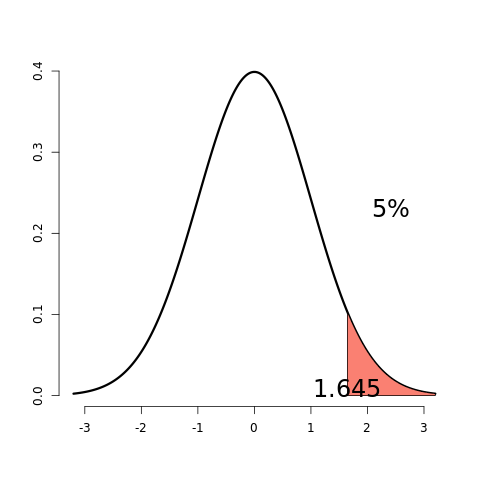
\includegraphics[scale=0.5]{figs/95th quantile of a gaussian.png}
    \caption{R-generated plot of the standard normal distribution $\mathcal{N}(0,1)$,  in the [-3.2, 3.2] range. The shaded polygon represents the 95th quantile (which is given by $x=1.645$) of a standard normal distribution. }
    \label{fig:my_label}
\end{figure}

In general, we don't convert $C$ back to its original scale. We would just reject it because the Z-score, how many standard error units the sample mean is above the hypothesised mean, is greater than $1.645$ \textit{ie. }

$$
\frac{32-30}{10/\sqrt{100}} = 2 > 1.645.
$$

We can codify these rules for a normal Z test as follows:

Let $H_0 : \mu = \mu_0$ be the null hypothesis, then let 
\begin{itemize}
    \item $H_1: \mu < \mu_0$
    \item $H_2: \mu \neq \mu_0$
    \item $H_1: \mu > \mu_0$
\end{itemize}

\end{document}
